\documentclass{minimal}
\usepackage{tikz}
\usetikzlibrary{shadings}
\begin{document}

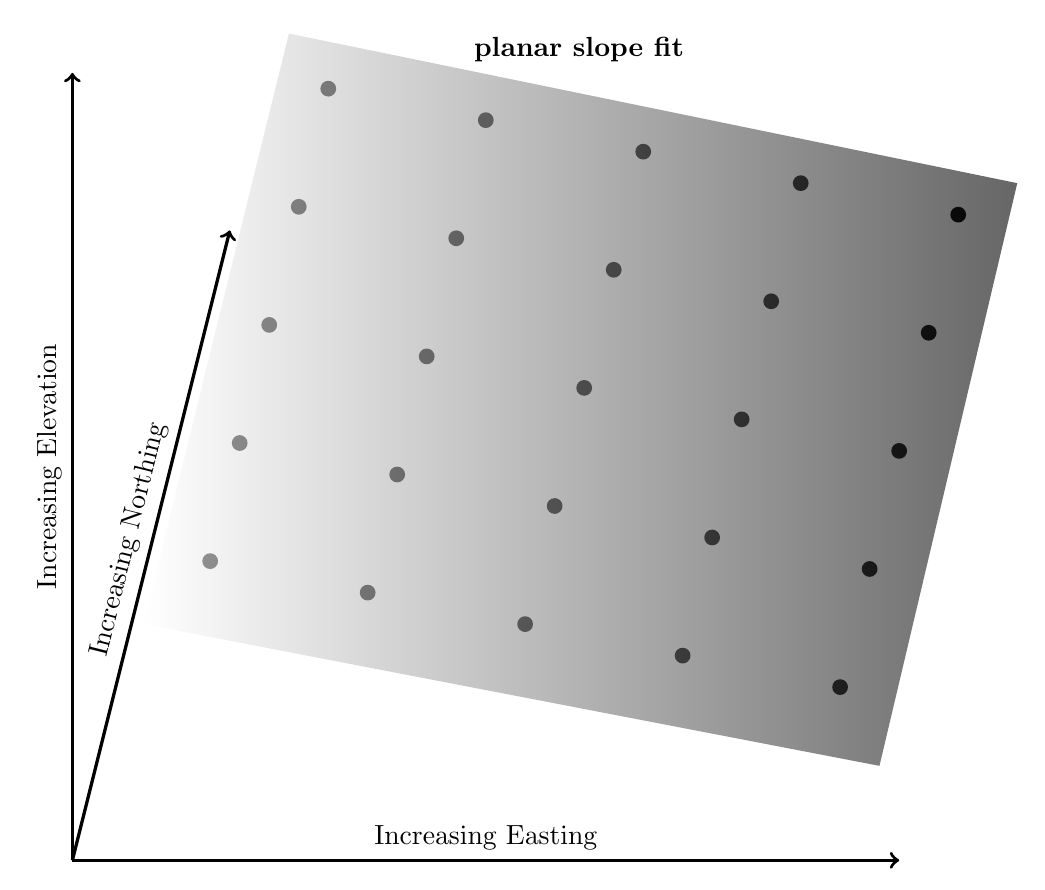
\begin{tikzpicture}

%draw external reference
\draw[->,black,very thick] (-0.5,0)--(-0.5,10) node[midway,above,sloped]{Increasing Elevation};
\draw[->,black,very thick] (-0.5,0)--(10,0) node[midway,above,sloped]{Increasing Easting};
\draw[->,black,very thick] (-0.5,0)--(1.5,8) node[midway,above,sloped]{Increasing Northing};

%label figure
\node[above right] at (current bounding box.north) {\textbf{planar slope fit}};

%draw points for visual
\foreach \x in {1,3,5,7,9}
	\foreach \y in {1,2.5,4,5.5,7} 
       {
    	\fill (\x  + \y*.25,\y + 3 - \x*.2) circle (0.1);
    	}

%draw slope rectangle
\shade[lower right=black, upper right=black, lower left=white, upper left=white, opacity=0.6] (0.4,3) -- (2.25,10.5) -- (11.5,8.6) -- (9.75,1.2) -- cycle;
		
\end{tikzpicture}
\end{document}